\section{综合}

\title[第7讲\quad 综合]{第7讲\quad 综合} 
\author{}
\date{}

\begin{frame}
    \titlepage
\end{frame}

\setcounter{framecounter}{0}

\begin{frame}
    \stepcounter{framecounter}
    \frametitle{习题\theframecounter}
    \vspace*{-1cm}
    \textit{下列竖式中,相同汉字表示相同数字,不同汉字表示不同数字,且所有汉字对应的数字都不是 0,2,5。“空歌风度清”表示的五位数是\underline{\hbox to 20mm{}}.}
    \begin{figure}[H] 
        \centering
        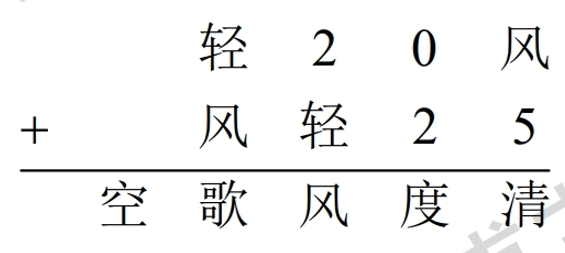
\includegraphics[width=0.4\textwidth]{./pics/Chapter_7/1.png}
    \end{figure}
    % 2025;16934
\end{frame}

\begin{frame}
    \stepcounter{framecounter}
    \frametitle{习题\theframecounter}
    \vspace*{-1cm}
    \textit{下面的算式中,相同的汉字代表相同的数字,不同的汉字代表不同的数字,那么\myoverline{龙行天下}  表示的四位数是\underline{\hbox to 20mm{}}.}
    \begin{figure}[H] 
        \centering
        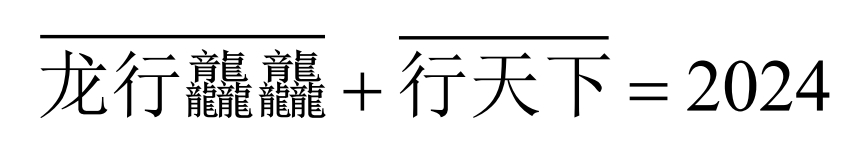
\includegraphics[width=0.4\textwidth]{./pics/Chapter_7/2.png}
    \end{figure}
    % 2024
\end{frame}

\begin{frame}
    \stepcounter{framecounter}
    \frametitle{习题\theframecounter}
    \textit{将 $1\sim 9$分别填入到右图的方框中,每个数字用一次,使得竖式成立;现在数字 6、7、8已经被填入,那么竖式的和是\underline{\hbox to 20mm{}}.}
    \begin{figure}[H] 
        \centering
        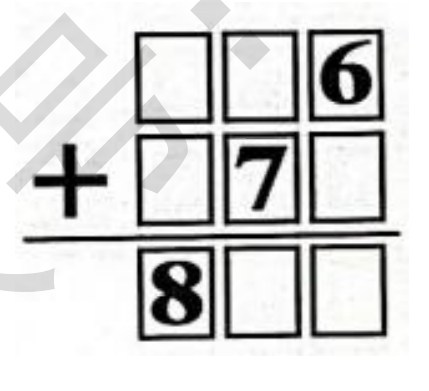
\includegraphics[width=0.3\textwidth]{./pics/Chapter_7/3.png}
    \end{figure}
    % 2023; 819
\end{frame}

\begin{frame}
    \stepcounter{framecounter}
    \frametitle{习题\theframecounter}
    \textit{老虎、狐狸、猴子各3只分别入住右图的9个房间中,每个房间一只,结果每只动物都说“有老虎与我相邻"(有公共边的两个房间相邻);如果老虎都说真话,狐狸都说假话,猴子说的话不知真假,那么说真话的猴子所在房间编号的和是\underline{\hbox to 20mm{}}.}
    \begin{figure}[H] 
        \centering
        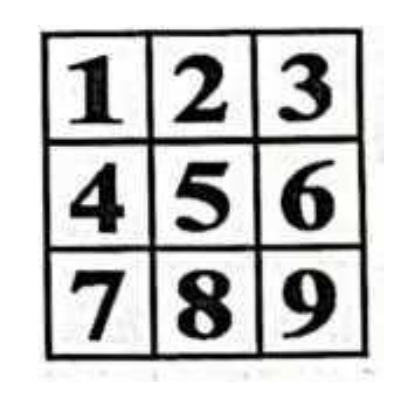
\includegraphics[width=0.3\textwidth]{./pics/Chapter_7/4.png}
    \end{figure}
    % 2023; 15
\end{frame}

\begin{frame}
    \stepcounter{framecounter}
    \frametitle{习题\theframecounter}
    \vspace*{-3cm}
    \textit{季老师将分别写有$1\sim 9$的九张卡片平均分给甲、乙、丙三人,每人只能看到自己的三张卡片(6 翻转后可以看成 9, 9 翻转后可以看成 6).甲说:你们的数都无法组成形如 ``AXB=C(A,B,C互不相同)'' 的乘法等式乙说:听了甲的话,我就知道甲手中的三个数分别是多少了如果他们都足够聪明且诚实,那么丙手中三个数的乘积是\underline{\hbox to 20mm{}}.}
    % 2024; 35
\end{frame}

\begin{frame}
    \stepcounter{framecounter}
    \frametitle{习题\theframecounter}
    \vspace*{-3cm}
    \textit{有一些自然数,如 121和 2552,从左到右和从右到左的数字顺序相同,我们把这样的自然数叫做“回文数”. 已知两个回文数的和是 2022,则这两个回文数的差是\underline{\hbox to 20mm{}}.}
    % 2022; 
\end{frame}


% \begin{frame}
%     \stepcounter{framecounter}
%     \frametitle{习题\theframecounter}
%     \textit{丽丽想用大小为 1x1、2x2、3x3 的三种正方形拼成下图所示的领奖台(图中每个小正方形的边长为1),所用正方形的面积总和为 15,且拼接过程中不可重叠,每种正方形数量不限(可以不用).共有\underline{\hbox to 20mm{}}种不同的拼接方法.(正方形的摆放位置或数量不同都算不同的拼法).}
%     \begin{figure}[H] 
%         \centering
%         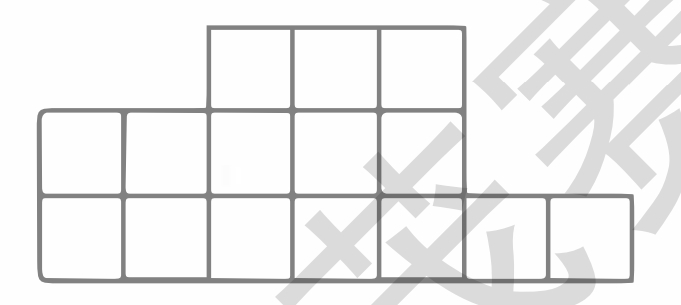
\includegraphics[width=0.4\textwidth]{./pics/Chapter_7/7.png}
%     \end{figure}
%     % 2022; 
% \end{frame}

\begin{frame}
    \stepcounter{framecounter}
    \frametitle{习题\theframecounter}
    \vspace*{-1cm}
    \textit{甲、乙、丙、丁四位绝世高手相约于华山之年比武论剑,争夺 ``天下第一'' 的名号. 四人抽签两两分组各自决出胜者,两位胜者再次比试决出一二名,两位败者决出三四名. 比武结束后四人进行了交流,每人说了两句话:\\
    甲: 我在与丙的大战中获得了胜利,但是成输给了丁.\\
    乙: 我作为天下第一实至名归,甲的名次比丙靠后.\\
    丙: 我被甲的六脉神剑击败了。乙在比试中输给了丁.\\
    丁: 好在我的名次没有垫底. 丙的名次比乙靠前.\\
    己知每个人在比试中胜了几场就说几句真话. 那么甲乙丙丁最终的名次按顺序组成的四位数为\underline{\hbox to 20mm{}}.}
    % 2022; 
\end{frame}


\begin{frame}
    \stepcounter{framecounter}
    \frametitle{习题\theframecounter}
    \vspace*{-3cm}
    \textit{在算式 $\overline{A0AA}= A\times B\times \overline{BBA}$中,A、B 分别代表不同的数字.那么, $\overline{AB}$ 代表的两位数是\underline{\hbox to 20mm{}}.}
    % 2022; 73
\end{frame}


\begin{frame}
    \stepcounter{framecounter}
    \frametitle{习题\theframecounter}
    \vspace*{-1cm}
    \textit{如图所示,正五边形的五个顶点位置分别标记为$1\sim 5$,甲乙丙戊分别站在了这五个不同的顶点上,发生如下对话:\\
甲对乙说:我所在位置上的数比你大. \\
乙对丙说:我所在位置上的数比你小. \\
丙对丁说:我所在位置上的数比你大. \\
丁对戊说:我所在位置上的数比你小. \\
戊对甲说:我所在位置上的数比你大. \\
如果五个人说的都是真话,且任意发生对话的两个人都不相邻. 那么甲乙丙丁戊所站位置按顺序连成的五位数是\underline{\hbox to 20mm{}}.}
    % 2022; 31425
\end{frame}


\begin{frame}
    \stepcounter{framecounter}
    \frametitle{习题\theframecounter}
    \textit{甲、乙二人按如下顺序填写下图中的减法算式:\\
    $\textcircled{1}$甲选择一个数字,然后乙选择一个位置将这个数字填入;\\
    $\textcircled{2}$甲选择一个之前没有选择过的数字, 然后乙选择一个位置将这个数字填入;\\
    $\textcircled{3}$甲选择一个之前没有选择过的数字, 然后乙将它填入    最后一个位置;\\
    如果甲希望两个数的差尽量大,乙希望这两个数的差尽量小,那么甲、乙都按照最佳策略填写算式时,差是\underline{\hbox to 20mm{}}.}
    \begin{figure}[H] 
        \centering
        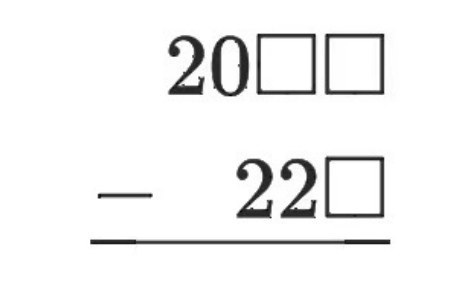
\includegraphics[width=0.2\textwidth]{./pics/Chapter_7/11.png}
    \end{figure}
    % 2022; 1854
\end{frame}


\begin{frame}
    \stepcounter{framecounter}
    \frametitle{习题\theframecounter}
    \vspace*{-1cm}
    \textit{在右图的加法竖式中,6个汉字恰好代表6个连续的数字,那么,花园探秘 所代表的四位数是\underline{\hbox to 20mm{}}.}
    \begin{figure}[H] 
        \centering
        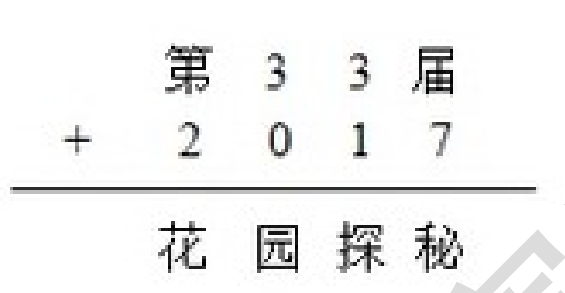
\includegraphics[width=0.4\textwidth]{./pics/Chapter_7/12.png}
    \end{figure}
    % 2021; 8354
\end{frame}


\begin{frame}
    \stepcounter{framecounter}
    \frametitle{习题\theframecounter}
    \textit{甲乙丙丁四个人各有一些糖果,他们之间的对话如下:\\
    甲:如果把我的糖果数量变成和丙一样多,我们4人的平均数会减少2;\\
    乙:如果我的糖果数量变成和丁一样多,我们4人的平均数会减半;\\
    丙:如果我的糖果数量变为原来2倍,而甲的数量减半,我们4人的平均数会增加 2;\\
    丁:如果我的糖果数量变为原来2倍,而乙的数量减半,我们4人的平均数恰好会是一个整十数.
事实证明,他们4人中只有糖果数量最少的人说了假话,并且糖果最多人的糖果数恰好是糖果最少人糖果数的3倍.那么,他们4人一共有\underline{\hbox to 20mm{}}颗糖果.}
    % 2021; 120
\end{frame}

\begin{frame}
    \stepcounter{framecounter}
    \frametitle{习题\theframecounter}
    \textit{在右面的乘法竖式中,相同的汉字代表相同的数字,不同的汉字代表不同的数字;那么,\myoverline{迎接夏天} 代表的四位数是\underline{\hbox to 20mm{}}.}
    \begin{figure}[H] 
        \centering
        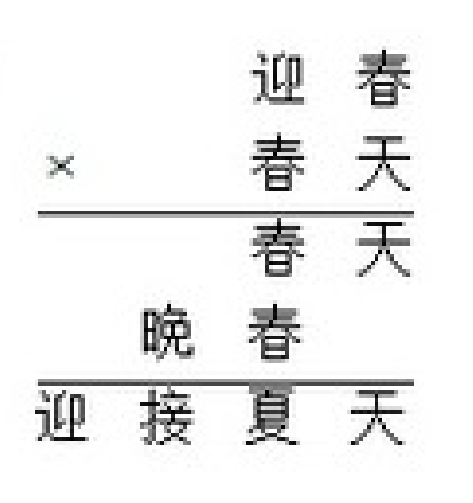
\includegraphics[width=0.4\textwidth]{./pics/Chapter_7/14.png}
    \end{figure}
    % 2021; 1024
\end{frame}

\begin{frame}
    \stepcounter{framecounter}
    \frametitle{习题\theframecounter}
    \vspace*{-1cm}
    \textit{甲、乙、丙、丁共有糖果 17颗,且每人的糖果数都不超过9颗,他们有如下的对话:\\
    甲对乙说:``如果我给你1颗糖,我们的糖果数就相同了.''\\
    乙对甲说:``如果你给我2颗糖,我的糖果数就是你的3倍了.''\\
    丙对甲说:``如果我给你3颗糖,你的糖果数就是我的3倍了.''\\
    丁对甲说:``如果你给我4颗糖,我的糖果数就是你的4倍了.''\\
    结果发现:糖果数是奇数的人说的都是对的,而糖果数是偶数的人说的都是错的.设甲、乙、丙、丁依次拥有 A、B、C、D颗,那么,四位数$\overline{ABCD}$是\underline{\hbox to 20mm{}}.}
    % 2021; 3158
\end{frame}